\documentclass[11pt,a4paper]{article}
\usepackage[utf8]{inputenc}
\usepackage[T1]{fontenc}
\usepackage{mathptmx}
\usepackage{amsfonts}
\usepackage{amsmath, amssymb}
\usepackage{bm}
\usepackage{nccmath}
\usepackage{graphicx}
\usepackage{titling}
\usepackage{indentfirst}
\usepackage{url}
\usepackage{xurl}
\usepackage[backend=biber,style=apa,date=year]{biblatex}
\usepackage{csquotes}
\usepackage{float}
\usepackage{sectsty}
\usepackage{enumitem}
\usepackage{hyphenat}
\usepackage{wrapfig}
\usepackage{hyperref}
\usepackage{enumitem}
\usepackage{titlesec}
\usepackage{authblk}
\usepackage[skip=0pt]{caption}
\DeclareSourcemap{
  \maps[datatype=bibtex]{
      \map{
        \step[fieldset=urldate, null]
      }
   }
}
\usepackage[top=0.5in, bottom=0.5in,left=1in,right=1in]{geometry} 
\addbibresource{Bio.bib}

\DeclareMathSymbol{\mh}{\mathord}{operators}{`\-}
\renewcommand{\thetable}{S\arabic{table}}
\renewcommand{\thefigure}{S\arabic{figure}}
\renewcommand{\theequation}{S\arabic{equation}}

\date{}

\begin{document}

\begin{center}
\Large
Implementing adaptive operating policies to achieve economic, and groundwater sustainability goals in agriculture using Evolutionary Multi-Objective Direct Policy Search \\ 
\vspace{0.5cm}
Supplemental Information 
\end{center}

\begin{center}
José M. Rodríguez-Flores$^{1,*}$, Rohini S. Gupta $^2$, Harrison B. Zeff $^3$,\\ Patrick M. Reed $^2$, Josué Medellín-Azuara $^1$\\
\end{center}

\begin{center}
\small
$^1$Environmental Systems Program, University of California Merced, CA, USA\\
$^2$Department of Civil and Environmental Engineering, Cornell University, NY, USA\\
$^3$Department of Environmental Sciences and Engineering, University of North Carolina at Chapel Hill, NC, USA\\
$^*$Corresponding Author: jrodriguezflores3@ucmerced.edu
\end{center}

\vspace{0.2cm}

\section{Sustainable Management Criteria Definitions}

The Sustainable Management Criteria (\cite{dwr_sustainable_2017}) defines:

\begin{itemize}
    \item \textit{Sustainable groundwater management as the management and use of groundwater in a manner that can be maintained during the planning and
    implementation horizon without causing undesirable results.}
    \item \textit{Measurable objectives as the specific, quantifiable goals for the maintenance or improvement of groundwater conditions that have been included in an adopted Plan.}
    \item \textit{The minimum threshold is the quantitative value that represents the groundwater condition in each representative monitoring well site that when exceeded, may cause an undesirable result.}
\end{itemize}

\section{Cropland Evolution Semitropic}

\begin{figure}[H]
    \centering
    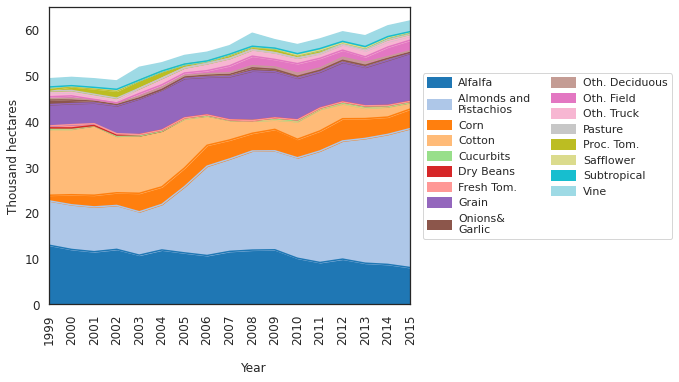
\includegraphics[width=0.8\textwidth]{land_hist_semitropic.png}
    \caption{Historical cropland of Semitropic WSD}
    \label{fig:m1esh1}
\end{figure}

\section{Surface Water Deliveries}

\begin{figure}[H]
    \centering
    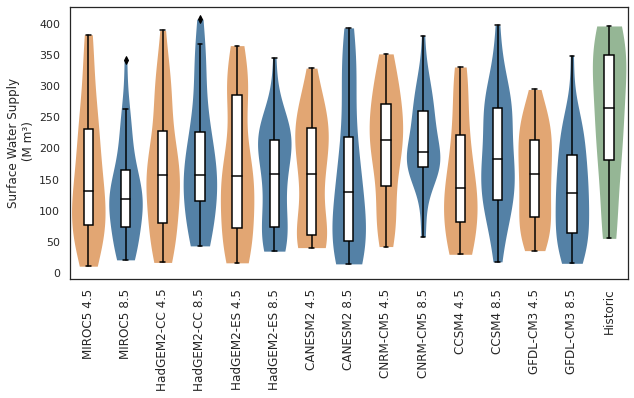
\includegraphics[width=0.7\textwidth]{gcm_surface_water.png}
    \caption{Distribution of historical (1999-2015) and surface water deliveries from CALFEWS (2016-2045) used in this study} \label{fig:SWSemitropic}
\end{figure}

\section{Calibrated Hydro-Economic Model Performance}

The following figures show the performance from running dynamically the coupled hydro-economic model with the last set of calibration parameters obtained from the data assimilation process (with 400 samples) over historical water available conditions. The model was let free to optimize land and water allocation decisions to assess its performance to replicate observed conditions. 

\begin{figure}[H]
\centering
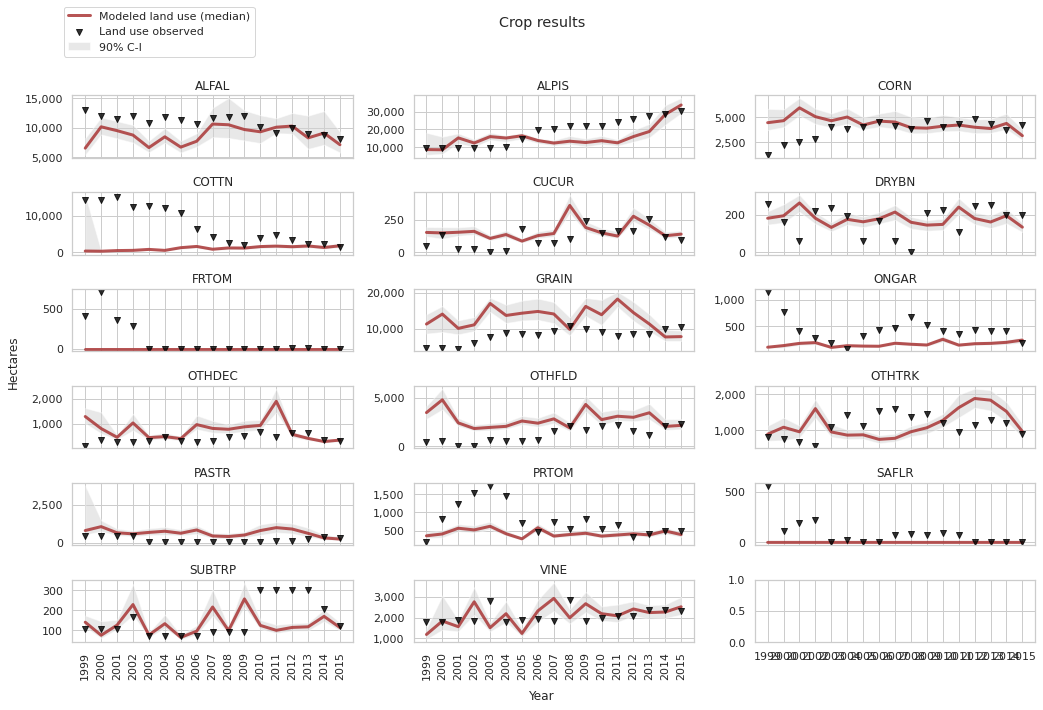
\includegraphics[width=1\textwidth]{land_use.png}
\label{fig:mesh1}
\caption{Land allocation from Hydro-economic model and observed}
\end{figure}

\begin{figure}[H]
\centering
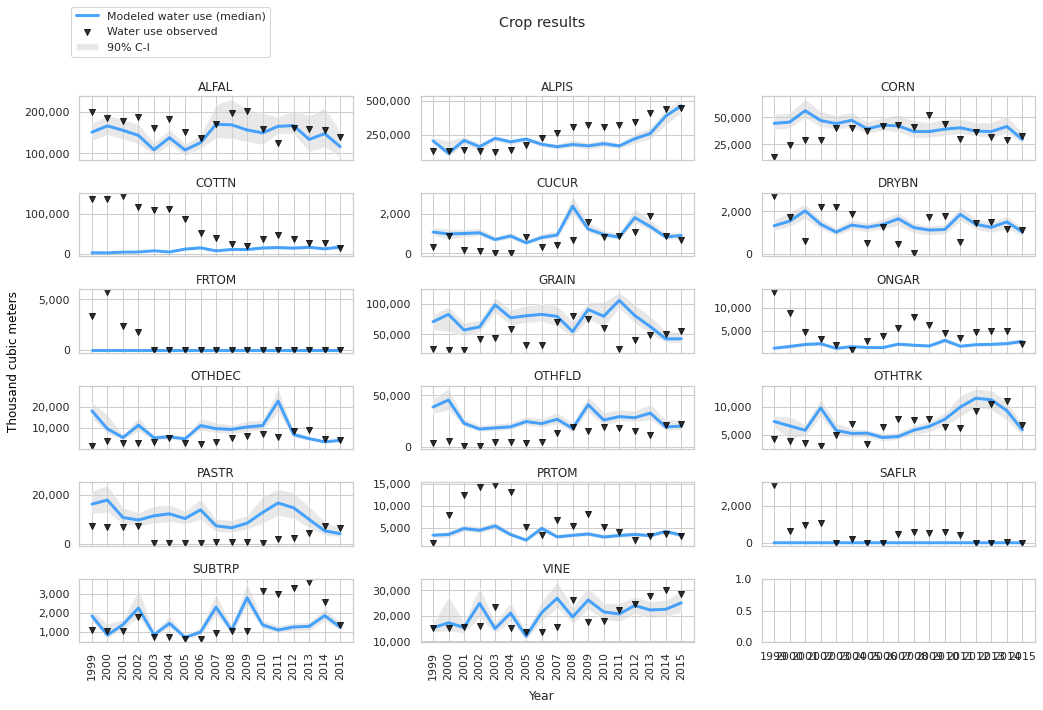
\includegraphics[width=1\textwidth]{water_use.png}
\label{fig:mesh1}
\caption{Water allocation from Hydro-economic model and observed}
\end{figure}

\begin{figure}[H]
\centering
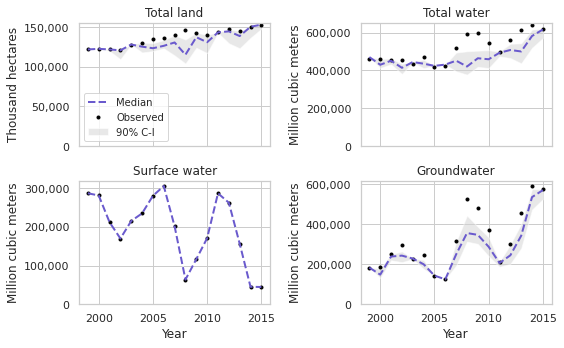
\includegraphics[width=0.8\textwidth]{water_use_by_source.png}
\label{fig:mesh1}
\caption{Total water allocation by source from Hydro-economic model and observed}
\end{figure}

\begin{figure}[H]
\centering
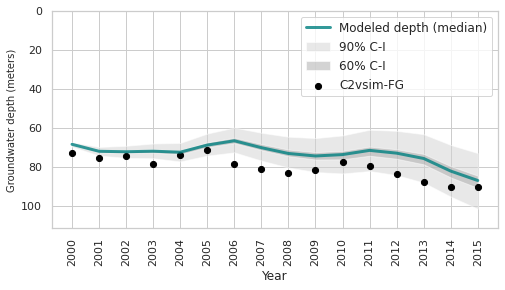
\includegraphics[width=0.6\textwidth]{gw_depth.png}
\label{fig:mesh1}
\caption{Simulated groundwater depth from running coupled hydro-economic model dynamically  and observed groundwater depth from \textcite{dwr_c2vsimfg_2021}}
\end{figure}


\section{Yield Elasticity to Water Use}

Crop yield elasticity to water ($\tilde{y}_{i,water}$) represents the response of yield to changes in water applied, as percent change in yield to a percent change in applied water. To estimate this parameter we used two approaches, first for crops Alfalfa, Corn, Almonds (in Almonds and Pistachios category), and Wheat (in Grain category) we used the VIC-CropSyst model (\cite{malek_viccropsyst-v2_2017}) calibrated for a spatial grid in the study area and using different irrigation systems. Crop yield responses were estimated by reducing applied water (deficit irrigation), responses from VIC-CropSyst (V-CS) were later used to estimate the crop yield water elasticity ($\tilde{y}_{i,water}$) using following a sigmoidal yield response function (Equation S1) described by \textcite{merel_regional_2014}. We fitted the sigmoidal response function using a nonlinear regression solving for $\alpha_{i,1},\alpha_{i,2},\alpha_{i,3}$. With the estimates from solving this regression the crop-specific yield response to water changes was later calculated using Equation S2. using the reference water applied ($\tilde{x}_{i,water}$) and reference yield ($\tilde{y}_{i}$) used in the PMP calibration (average of the historical). 

\begin{flalign}
\hat{y}_{i,V-CS} = \dfrac{\alpha_{i,1}}{1 + exp\left(-\dfrac{\hat{x}_{i,water,V-CS}-\alpha_{i,2}}{\alpha_{i,3}}\right)}
\end{flalign}

\begin{flalign}
\tilde{y}_{i,water} = \dfrac{\tilde{x}_{i,water}exp\left(-\dfrac{\tilde{x}_{i,water}-\bar{\alpha}_{i,2}}{\bar{\alpha}_{i,3}}\right)\hat{y}_{i}}{\bar{\alpha}_{i,1}\bar{\alpha}_{i,3}}
\end{flalign}

For the rest of the crops we used the applied water by crop category from \textcite{dwr_agricultural_2020} and yield from the most representative crop within each group using the land reported by \textcite{usda_national_2020}, both reported at a county level and using the data from 1998 to 2015. We estimated the elasticity through least squares (Equation S3) as the slope between the natural logarithm of production and the natural logarithm of water used. We compared our results with other published values for crops in California, specially for San Joaquin Valley (\cite{garnache_social_2017,merel_regional_2014}). 

\begin{flalign}
ln(\tilde{y}_{i,t}) = \tilde{y}_{i,water}ln(\tilde{x}_{i,water,t})
\end{flalign}

\section{Groundwater Depth Response}

\begin{figure}[H]
\centering
    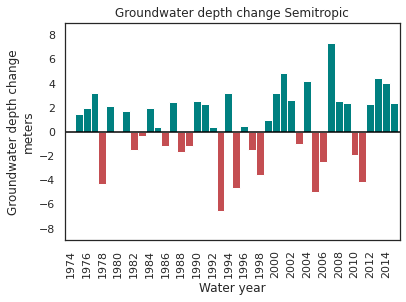
\includegraphics[width=0.6\textwidth]{Depth_change_semitropic}
    \label{fig:mesh1}
    \caption{Changes on distance to groundwater depth from C2VSIM-FG}
\end{figure}

Using groundwater pumping of the year $t$ and $t-1$ and water year type (Wet, Normal and Dry) of the year $t$ and $t-1$ as index variables we fitted different Bayesian linear modes. Pooled model (or fixed-effects) assigns same model parameters (intercept and slopes) across water year types. Un-pooled model assigns different parameters to each water year type as if water-year type is independent and have different intercepts and slopes. Finally, the Hierarchical model (or random-effects or multi-level) assigns different parameters to each water-year type varying intercepts or slopes (or both) across water-year type categories, this models enables the statistical model to learn how the agricultural pumping affects the groundwater depth change in each water year type while learning this effect from all the water wear types at the same time. 

Groundwater pumping ($GWP_{t}$, $GWP_{t-1}$) and change of depth to groundwater ($\Delta{GWD}_t$) were normalized using the z-score normalization. Bayesian modeling uses a maximum entropy distribution to define the likelihood of the output, for this study we use Student's-t distribution to model the groundwater depth change probability distribution. The characteristics of the Student's t distribution makes it a more robust distribution to include extreme values and that can improve the MCMC sampling process. Additionally we need to define priors of the parameters (or unobserved variables). For this study we defined Gaussian priors for the intercept and slopes in all the model variations. As we expect that the relationship between groundwater depth change and change being positive for which case we centered the Gaussian distribution on the positive side for ${GWP}_t$ and a less informative distribution centered in 0 for ${GWP}_{t-1}$. Additionally an exponential distribution for the standard deviation priors  and Gamma distribution for the degrees of freedom of the Student-t's distribution prior. 

\begin{itemize}[noitemsep,topsep=4pt]
  \item P1: Pooled,   $\mu_t = \alpha + \beta_{1}GWP_{t}$
  \item P2: Pooled with lag on pumping,   $\mu_t = \alpha + \beta_{1}GWP_{t} + \beta_{2}GWP_{t-1} $
  \item U1: Unpooled, $\mu_t = \alpha_{WY_{t}} + \beta_{1,WY_{t}}GWP_{t}$
  \item U2: Unpooled with lag on pumping, $\mu_t = \alpha_{WY_{t}} + \beta_{1,WY_{t}}GWP_{t} + \beta_{2,WY_{t}}GWP_{t} $
  \item U3: Unpooled with lag on pumping and slope, $\mu_t =  \alpha_{WY_{t}} + \gamma_{WY_{t-1}} + \beta_{1,WY_{t}}GWP_{t} + \beta_{2,WY_{t}}GWP_{t}$
  \item H1: Hirerarchical with varying intercept, $\mu_t = \alpha_{WY_{t}} + \beta_{1}GWP_{t}$
  \item H2: Hirerarchical with varying intercept and varying slope, $\mu_t = \alpha_{WY_{t}} + \beta_{1,WY_{t}}GWP_{t}$
  \item H3: Hirerarchical with varying slopes, $\mu_t = \alpha_t + \beta_{1,WY_{t}}GWP_{t} + \beta_{2,WY_{t}}GWP_{t}$
  \item H4: Hirerarchical with varying intercept and slopes, $\mu_t = \alpha_{WY_{t}} + \beta_{1,WY_{t}}GWP_{t} + \beta_{2,WY_{t}}GWP_{t}$
  \item H5: Hirerarchical with varying intercepts and slopes, $\mu_t = \alpha_{WY_{t}} + \gamma_{WY_{t-1}} + \beta_{1,WY_{t}}GWP_{t} + \beta_{2,WY_{t}}GWP_{t}$
\end{itemize}

Model variations include pooled, un-pooled and hierarchical models, using the Water Year Type as index variable. Models were fit using a Markov Chain Monte Carlo (MCMC) sampling method using the probabilistic programming Python package PyMC (\cite{salvatier_probabilistic_2016}). Model selection was done using the Leave-one-out Cross-validation (LOO-CV) as estimate of the out-of-sample predictive fit (\cite{vehtari_practical_2017}), selecting the model with the highest log-scale LOO-CV or with he best out-of-sample prediction (Figure B2). The LOO-CV validation results are summarized in the Figure S8. Where the best model is the hirerarchical model with varying intercepts (H5), however the model with unpooled effects in intercepts and pumping (U3) was selected since is a simpler model and has a LOO close to H5. Hence, we obtain similar predictive power for a more computational efficient model. 

\begin{figure}[H]
\centering
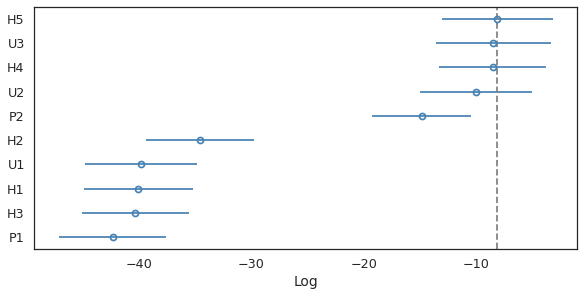
\includegraphics[width=0.7\textwidth]{model_comparison_calibration.png}
\label{fig:mesh1}
\caption{Leave-one-out cross-validation results}
\end{figure}

Table S1 shows the results from the model U3 summarizing the distribution of the posterior distribution of the parameters.

\begin{center}
\begin{tabular}{ |c|c|c|c|c| }
 \hline
 Parameter & Mean & Sd & HDI $2.5\%$ & HDI $97.5\%$ \\ 
 \hline
$\alpha_{1[Wet_{t}]}$ & 	-0.063 &	0.232 &	-0.478 &	0.405 		 \\
$\alpha_{1[Normal_{t}]}$ & 0.041 &	0.223 &	-0.379 &	0.501 	 \\
$\alpha_{1[Dry_{t}]}$ & 	 0.079 &	0.217 &	-0.356 &	0.494	 \\
$\gamma_{1[Wet_{t}]}$ & 	-0.057 	& 0.224 &	-0.481 &	0.393 	 \\
$\gamma_{1[Normal_{t}]}$ & 0.159 &	0.225 &	-0.285 &	0.588 \\
$\gamma_{1[Dry_{t}]}$ & -0.041 &	0.217 &	-0.453 &	0.400 	 \\
$\beta_{1[Wet_{t \mh 1}]}$ & 1.207 &	0.107 &	0.995 &	1.419 	 \\
$\beta_{1[Normal_{t \mh 1}]}$ 	& 0.829 &	0.148 &	0.550 &	1.126	\\
$\beta_{1[Dry_{t \mh 1}]}$ & 0.817 &	0.088 &	0.649 &	0.991 \\
$\beta_{2[Wet_{t \mh 1}]}$ & -0.757 	& 0.100 & -0.940 & 	-0.551 	 \\
$\beta_{2[Normal_{t \mh 1}]}$ & -0.807 &	0.141 &	-1.094 & -0.543 	\\
$\beta_{2[Dry_{t \mh 1}]}$ & -0.336 	& 0.088 & 	- 0.507 &  -0.159 \\
$\sigma$ & 0.235 & 	0.037 & 0.169 & 	0.310 \\
$\nu$ 	& 20.470 & 	12.859 & 2.469 &  	45.244 \\
\hline
\end{tabular}
\captionof{table}{Marginal posterior distributions of the parameters of Groundwater Depth Response}
\end{center}

\begin{figure}[H]
\centering
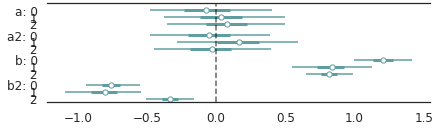
\includegraphics[width=0.7\textwidth]{gw_depth_response_posterior_2.png}
\label{fig:mesh1}
\caption{Posterior Distributions of the parameters, where 0 is Wet Year, 1 is Normal Year and 2 is Dry Year}
\end{figure}

\section{Borg Epsilon values and Hypervolume from Random Seeds}

\begin{center}
\begin{tabular}{ |c|c| }
 \hline
 Objective & Epsilon \\ 
 \hline
Maximize Average Total Revenues (O1) & 30  \\
Minimize Average Groundwater Depth (O2) & 1.8 \\
Maximize 5th Percentile Revenue in a year (O3) & 1 \\
Minimize 95th Groundwater Depth Change in a year (O4) & 0.9 \\
Reliability (O5) & 0.01 \\
\hline
\end{tabular}
\captionof{table}{Epsilon values used for the Borg MOEA}
\end{center}

\begin{figure}[H]
    \centering
    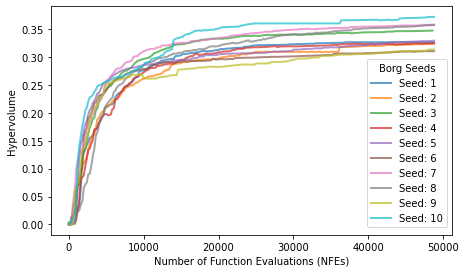
\includegraphics[width=0.9\textwidth]{Borg_Seeds_Hypervolume.png}
    \caption{Hypervolume from 10 random seeds used in Borg MOEA}
    \label{fig:m1esh1}
\end{figure}

\section{Performance selected Robust Policies}

\begin{figure}[H]
    \centering
    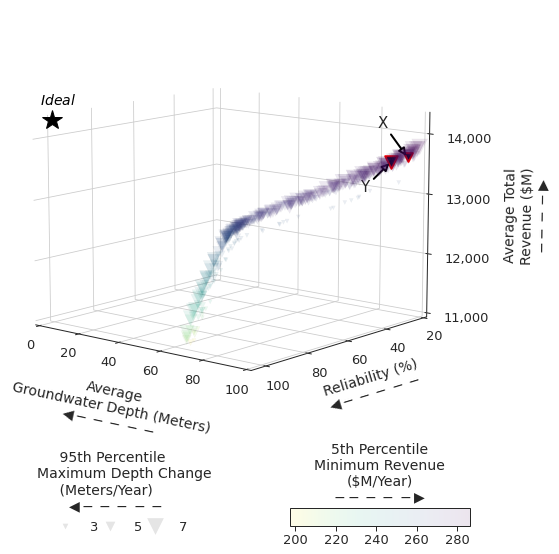
\includegraphics[width=0.7\textwidth]{3d_selected_robust.png}
    \caption{Selection of three Robust Policies}
    \label{fig:m1esh1}
\end{figure}


\begin{center}
\begin{tabular}{ |c|c|c|c|c|c| }
 \hline
 Solution & O1 & O2 & O3 & O4 & O5 \\ 
 \hline
X &  13,620  & 96.62 & 283.51 & 4.3 & 23.7\% \\
Y & 13,441 & 95.4 & 282 & 5.5 & 31\% \\
\hline
\end{tabular}
\captionof{table}{Performance of the selected Robust Policies shown in Figure S11}
\end{center}


\begin{figure}[H]
    \centering
    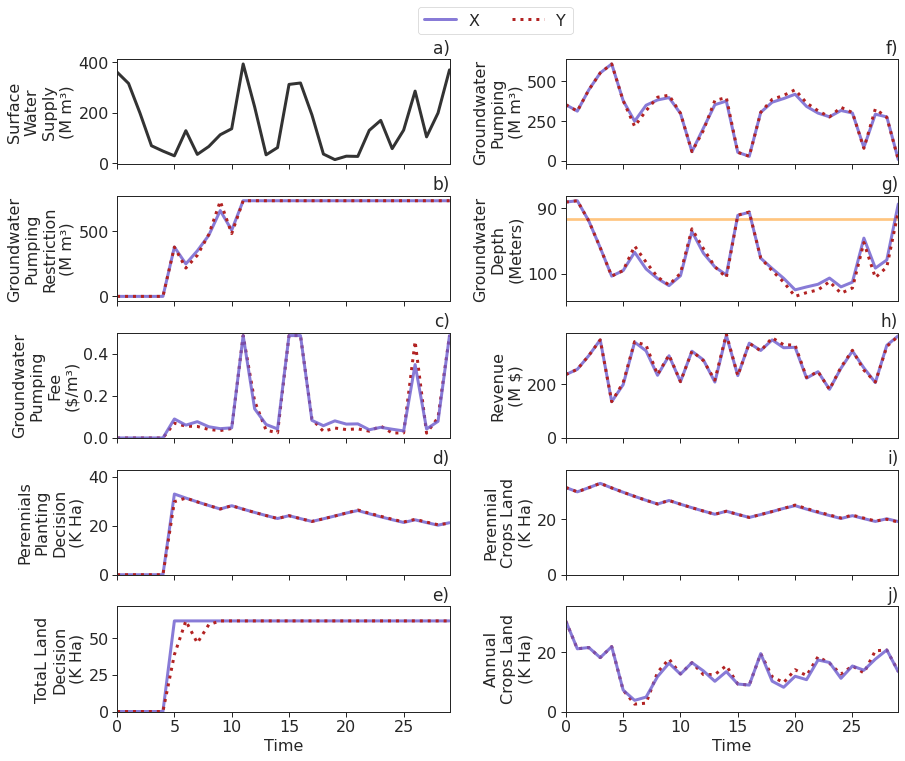
\includegraphics[width=1\textwidth]{selected_robust_performance_s1.png}
    \caption{Performance Robust Policies under largest standard deviation surface water deliveries (CANESM2 8.5). Sub-figure (a) shows the surface water deliveries.Sub-figures (b) to (e) show the dynamic decisions in the control policy. Sub-figures (f) to (j) show the performance of the food-water system. The orange line in Sub-figure (g) depicts the measurable objective used in the experiment}
    \label{fig:m1esh1}
\end{figure}


\begin{figure}[H]
    \centering
    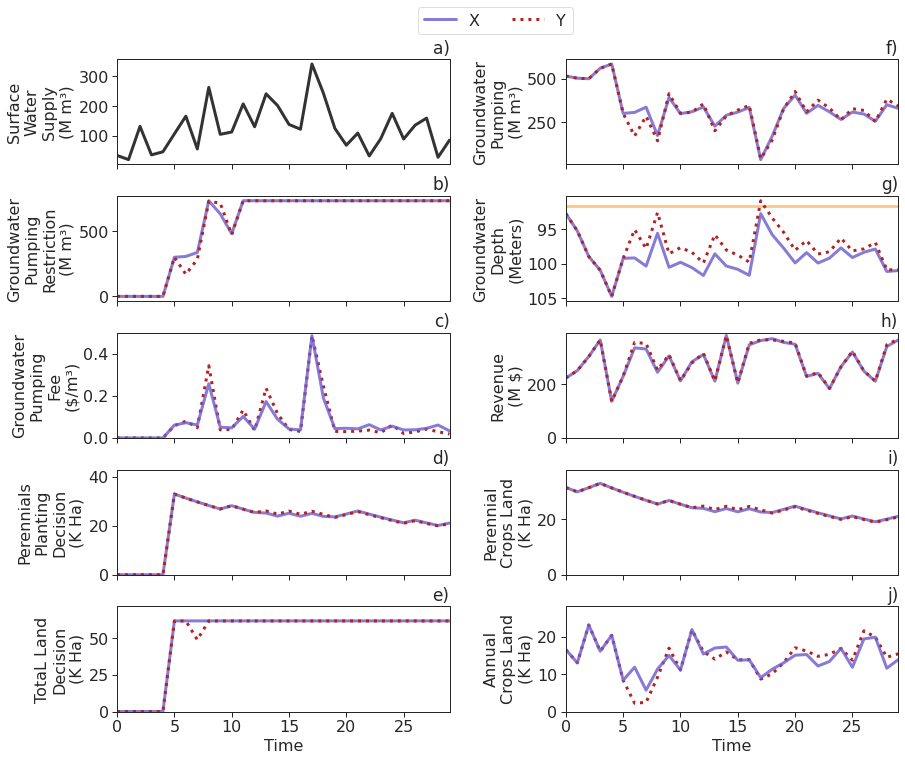
\includegraphics[width=1\textwidth]{selected_robust_performance_s2_dry.png}
    \caption{Performance Robust Policies under driest average surface water deliveries (MIROC 8.5). Sub-figure (a) shows the surface water deliveries.Sub-figures (b) to (e) show the dynamic decisions in the control policy. Sub-figures (f) to (j) show the performance of the food-water system. The orange line in Sub-figure (g) depicts the measurable objective used in the experiment}
    \label{fig:m1esh1}
\end{figure}



\begin{figure}[H]
    \centering
    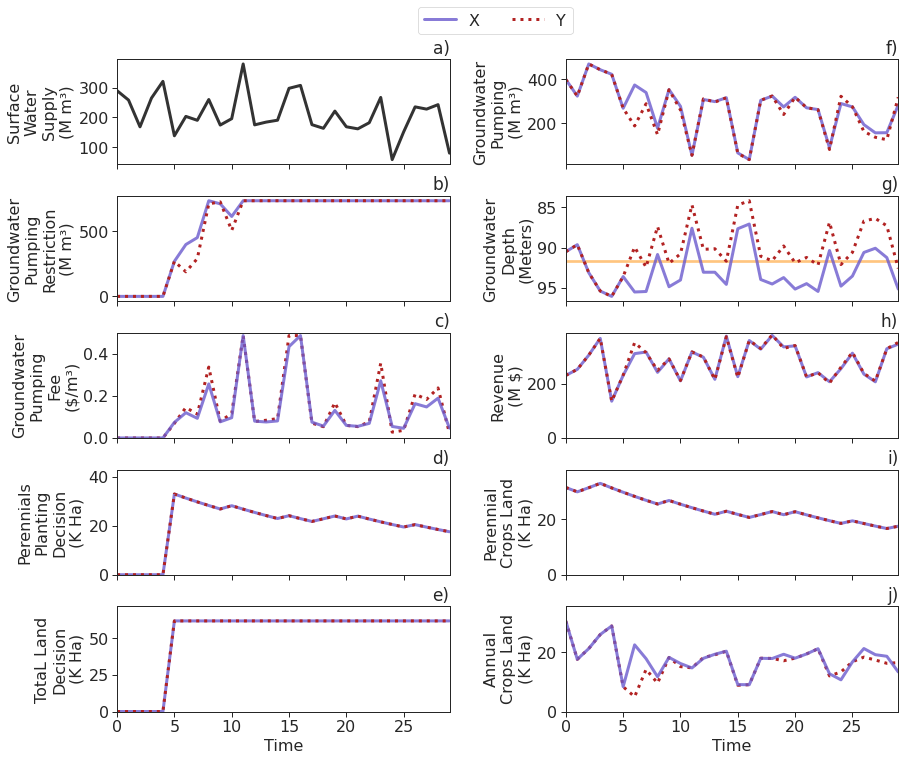
\includegraphics[width=1\textwidth]{selected_robust_performance_s2_wet.png}
    \caption{Performance Robust Policies under largest (wet) average surface water deliveries (CNRM-CM5 8.5). Sub-figure (a) shows the surface water deliveries.Sub-figures (b) to (e) show the dynamic decisions in the control policy. Sub-figures (f) to (j) show the performance of the food-water system. The orange line in Sub-figure (g) depicts the measurable objective used in the experiment}
    \label{fig:m1esh1}
\end{figure}






\newpage
\printbibliography

\end{document}
